\documentclass{beamer}
\usepackage[T1]{fontenc}
\usepackage[utf8]{inputenc}
\usepackage[slovene]{babel}
\usepackage{pgfpages}           % privat zapiski
\usepackage{amsfonts}
\usepackage{amsmath,amsthm}     % pravilen izpis v "math mode"
%\usepackage{hyperref}
\usepackage{graphicx}           % za slike
\usepackage{multicol}
\usepackage{ulem}
\usepackage{bibentry}
\usepackage{caption}
\usepackage{subcaption}
\usepackage{algpseudocodex}
\usepackage{tikz}
\usepackage{booktabs}
\usepackage[table]{xcolor}
\usetikzlibrary{shapes,calc,positioning,arrows,arrows.meta, positioning, trees, shapes.geometric, tikzmark, shadows}

%\hypersetup{hidelinks}

\setbeamertemplate{theorems}[ams style]             % numbered da brez bold 

\setbeameroption{hide notes}                        % samo prosojnice
%\setbeameroption{show only notes}                   % samo zapiski
% \setbeameroption{show notes on second screen=right}  % oboje

\usepackage{palatino}
\usefonttheme{serif}

%\usecolortheme{beetle} %ali beetle morda ali seagull

\beamertemplatenavigationsymbolsempty
\setbeamertemplate{footline}[frame number]{} % oštevilčenje
\setbeamertemplate{note page}{\pagecolor{yellow!5}\insertnote}

\newtheorem{izrek}{Izrek}
\newtheorem{trditev}[izrek]{Trditev}
\newtheorem{posledica}[izrek]{Posledica}
\newtheorem{definicija}[izrek]{Definicija}
\newtheorem{naloga}[izrek]{Naloga}
\newtheorem{resitev}[izrek]{Naloga}

\definecolor{good}{HTML}{C8E6C9} % A light green
\definecolor{ok}{HTML}{FFF9C4}   % A light yellow
\definecolor{bad}{HTML}{FFCDD2}  % A light red

\author{Tim Kalan \\ \medskip
        \footnotesize Mentor: doc.~dr. Tilen Marc}
% \author{Tim Kalan}
        \institute[FMF]{Fakulteta za matematiko in fiziko \\
        Fakulteta za računalništvo in informatiko}
\title{
    Večstranski Schnorrovi podpisi \\
    \large (angl. \textit{Schnorr multisignatures})}
% \title{Večstranski Schnorrovi podpisi}
\date{10. oktober 2025} 

\begin{document}

\begin{frame}
    \titlepage
    \note[item]{15 s}
    \note[item]{Pozdravljeni, moje ime je Tim Kalan in ...}
    \note[item]{Šala?}
\end{frame}

\begin{frame}
    \frametitle{Vsebina}
    % \framesubtitle{Pregled predstavljenih tematik}
    \note[item]{15 s}
    \begin{enumerate}
        \item \textbf{Motivacija}
        \note[item]{Uvod: Zakaj sploh potrebujemo večkratne podpise in katere probleme rešujejo?}
        \item \textbf{Osnova}: Schnorr
        \note[item]{Teoretična osnova: Predstavitev Schnorrovega podpisnega algoritma.}
        \item \textbf{Prvi pristop}: ASM
        \note[item]{Analiza sheme ASM, njen potek in varnostni model.}
        \item \textbf{Drugi pristop}: MuSig2
        \note[item]{Predstavitev sodobne in učinkovitejše sheme MuSig2.}
        \item \textbf{Empirična analiza}
        \note[item]{Primerjava zmogljivosti, hitrosti in velikosti podpisov obeh pristopov.}
    \end{enumerate}
\end{frame}

\begin{frame}
    \frametitle{Podpisovanje v skupini}
    % \framesubtitle{Podpisovanje v skupini}
    \begin{columns}
        \begin{column}{0.5\textwidth}
            \begin{figure}
                \centering
                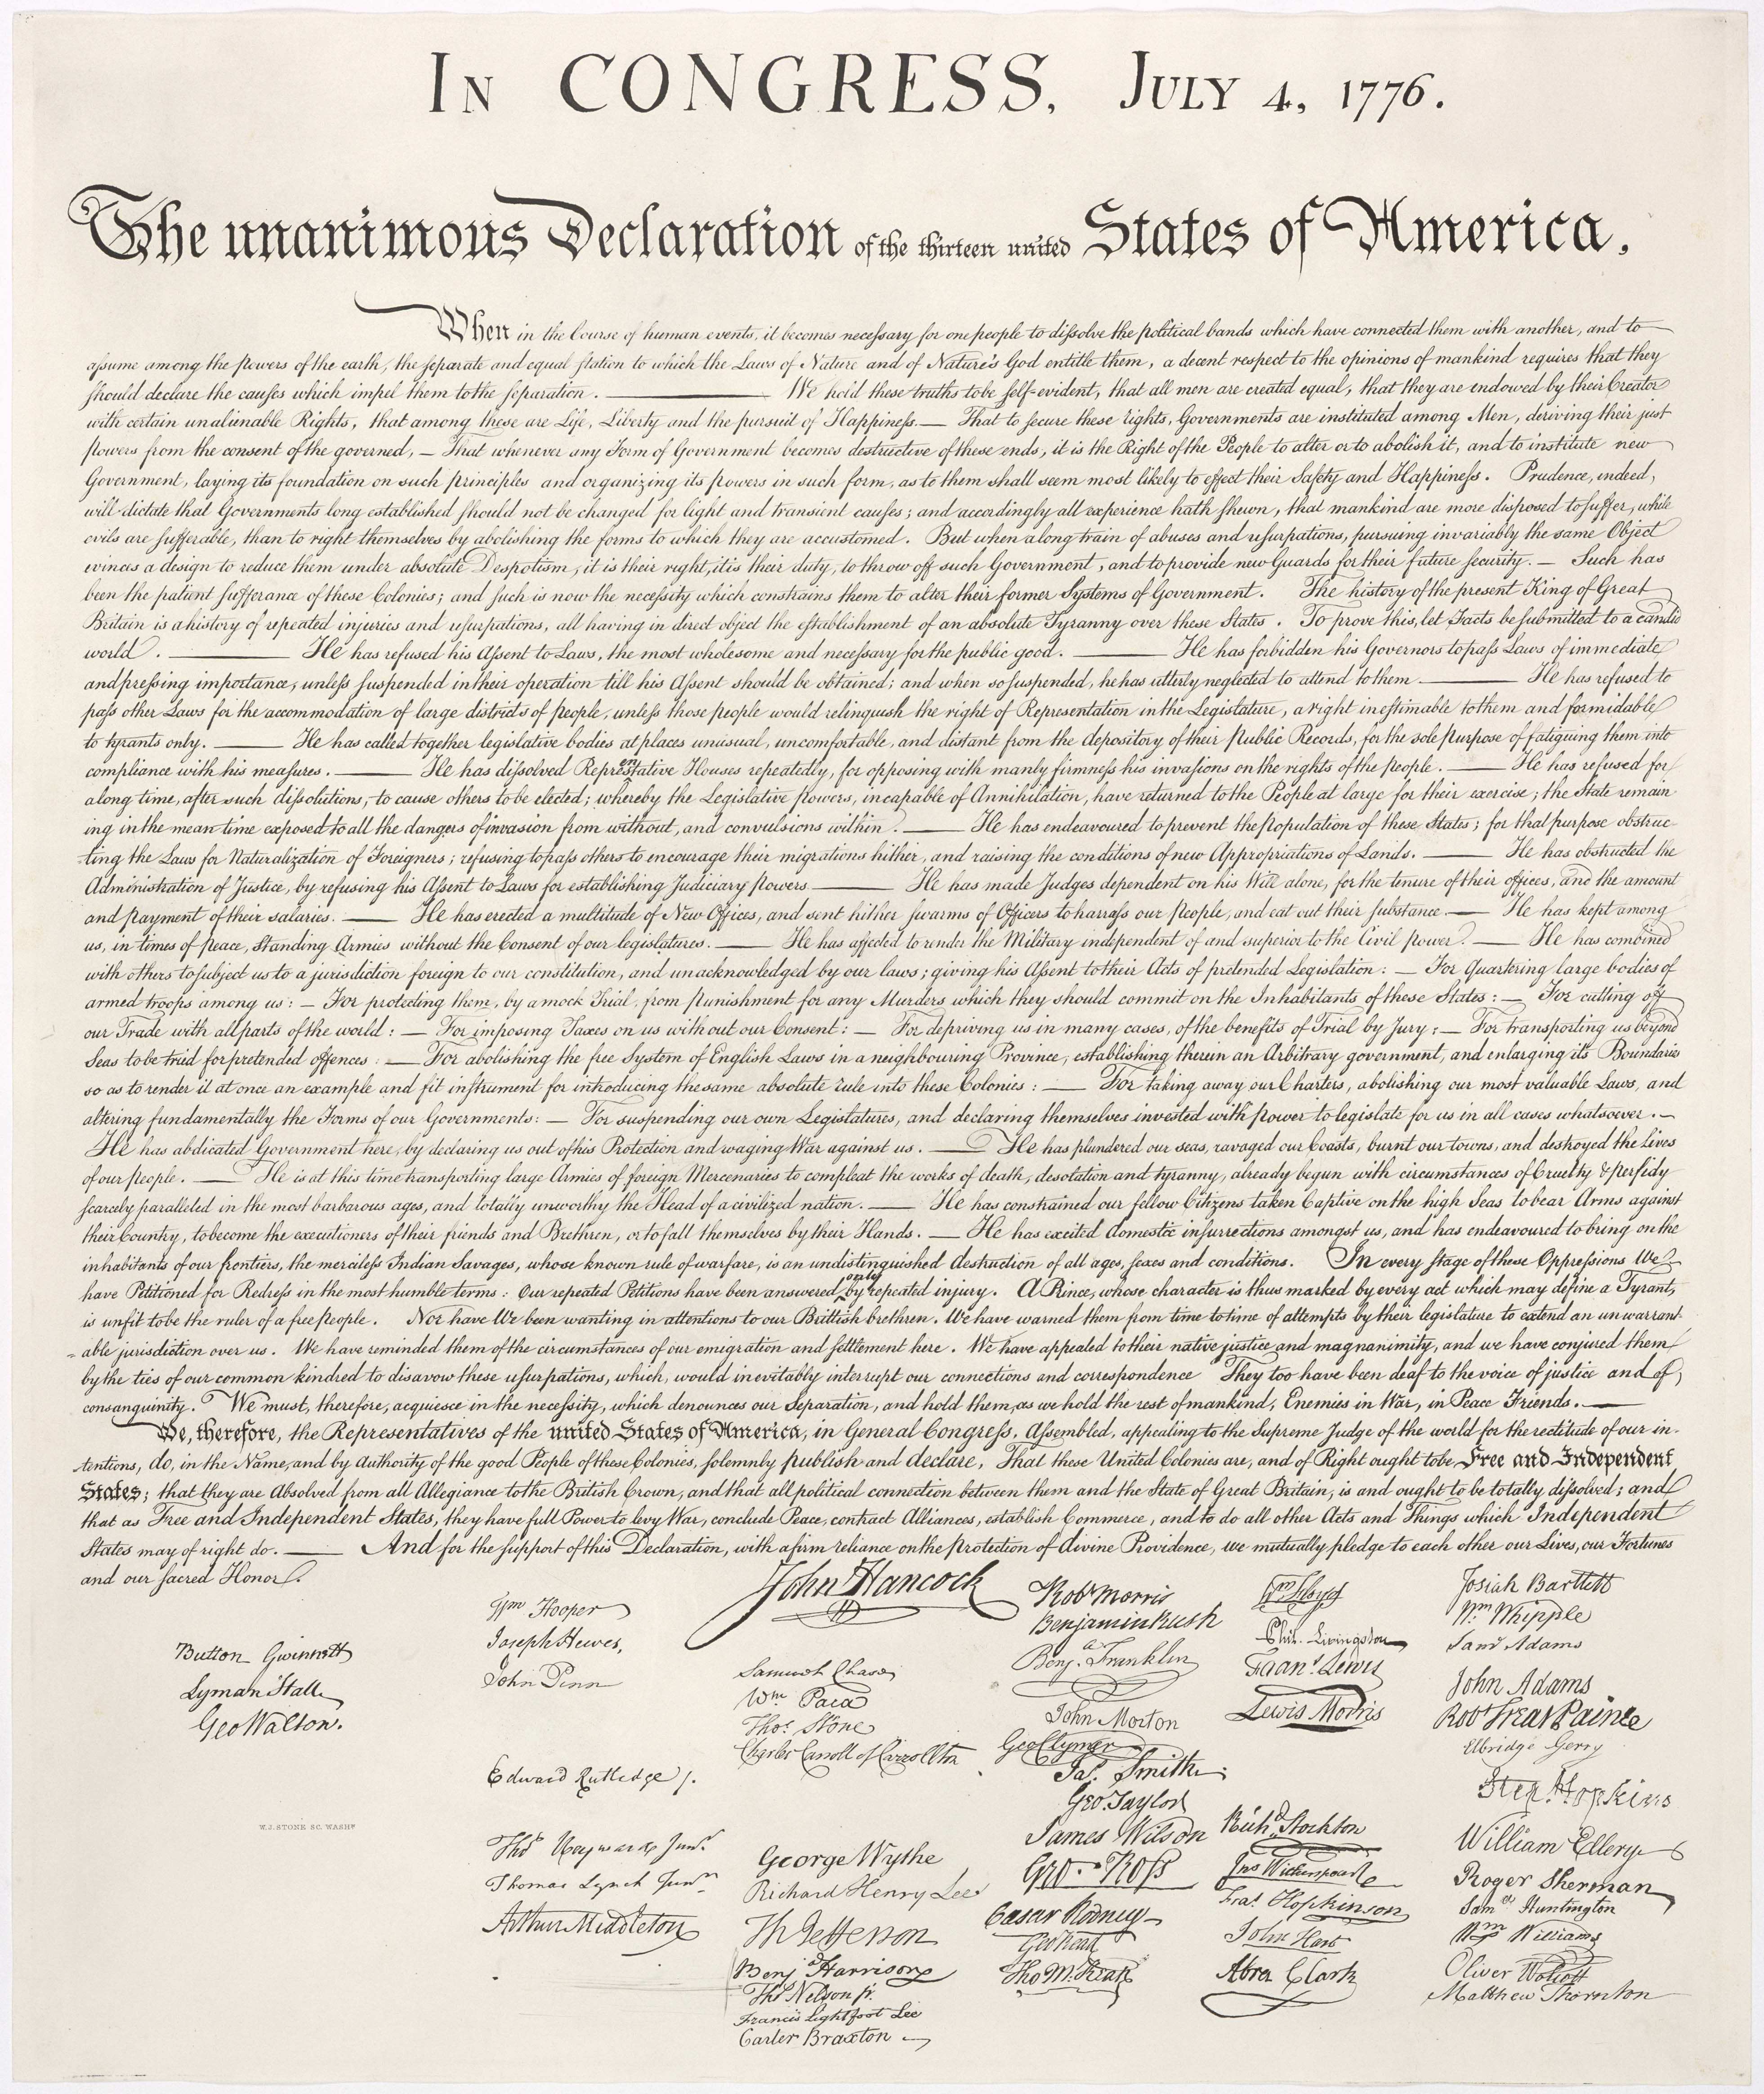
\includegraphics[width=\textwidth]{images/declaration.jpg}
                \tiny Deklaracija neodvisnosti ZDA
            \end{figure}
        \end{column}
        \begin{column}{0.5\textwidth}
            \textbf{Problem:} Nizanje podpisov.
            \begin{itemize}
                \item Velikost in čas preverjanja rasteta linearno.
            \end{itemize}
            \vspace{1cm}
            % \bigskip
            \textbf{Rešitev:} Večstranski podpisi.
             \begin{itemize}
                \item En sam podpis, hitro preverjanje.
            \end{itemize}
        \end{column}
    \end{columns}
    \note[item]{60 s}
    \note[item]{Že od nekdaj se srečujemo s situacijami, kjer mora nek dokument podpisati več oseb, kot na primer pri Deklaraciji neodvisnosti ZDA.}
    \note[item]{V digitalnem svetu je najbolj preprost pristop k temu preprosto zbiranje in nizanje posameznih digitalnih podpisov}
    \note[item]{Vendar ta pristop hitro postane zelo neučinkovit. Z vsakim novim podpisnikom se končni 'podpis' 
        podaljša, prav tako pa se podaljša čas, ki ga potrebujemo za preverjanje. Ta čas, kot bomo videli, narašča linearno.}
    \note[item]{To je še posebej problematično pri aplikacijah, kot je tehnologija veriženja blokov, kjer sta velikost in
        čas preverjanja neposredno povezana s ceno transakcije.}
    \note[item]{Moje delo se zato osredotoča na boljšo rešitev: večstranske podpise. To so kriptografske
        sheme, kjer celotna skupina ustvari en sam, kratek podpis, katerega preverjanje je hitro in učinkovito,
        ne glede na število podpisnikov.}
    \note[item]{V nadaljevanju bomo raziskali kompromis med odgovornostjo in učinkovitostjo, ki ga te
        sheme predstavljajo, in primerjali dva ključna pristopa: klasični večstranski Schnorrov podpis
        in sodobni protokol MuSig2}
\end{frame}

\begin{frame}
    \frametitle{Lastnosti idealnega večstranskega podpisa}
    % \framesubtitle{Kaj želimo doseči?}
    \vspace{0.5cm}
    \begin{itemize}
        \item \textbf{Učinkovitost}: Hitro preverjanje%: En sam, kratek podpis. Hitro preverjanje, neodvisno od števila podpisnikov.
        \item \textbf{Minimalna komunikacija}: Podpisniki se ne čakajo%: Čim manj krogov izmenjave sporočil med podpisniki.
        \bigskip
        \item \textbf{Odgovornost}: Kdo je naredil podpis?%: Možnost natančne identifikacije dejanskih podpisnikov.
        \item \textbf{Prilagodljivost}: Kdo lahko naredi podpis?%: Podpisovanje s strani poljubne podskupine članov.
    \end{itemize}
    \note[item]{60 s}
    \note[item]{Na prejšnjem slajdu smo videli, da je preprosto nizanje podpisov neučinkovito. Poglejmo si torej, kakšne so lastnosti idealne rešitve – idealnega večstranskega podpisa.}
    \note[item]{Prvič, želimo \textbf{učinkovitost}. To pomeni, da ne glede na to, ali dokument podpiše pet ali petsto članov, mora biti končni rezultat en sam, kratek podpis. Njegovo preverjanje mora biti enako hitro kot preverjanje navadnega, individualnega podpisa.}
    \note[item]{Drugič, želimo si \textbf{odgovornosti}. Preveritelj mora imeti možnost iz podpisa razbrati, kdo točno je sodeloval pri njegovem ustvarjanju. Je podpisal tudi direktor, ali samo ekipa pripravnikov?}
    \note[item]{Tretjič, pomembna je \textbf{prilagodljivost}. Shema mora omogočati, da veljaven podpis ustvari katerakoli podskupina. Morda za nek dokument potrebujemo podpise treh od petih članov upravnega odbora.}
    \note[item]{In končno, z vidika podpisnikov, želimo \textbf{minimalno komunikacijo}. Ker morajo podpisniki med postopkom med seboj izmenjevati podatke, je cilj, da je število teh komunikacijskih krogov čim manjše.}
    \note[item]{Kot bomo videli, je doseganje vseh teh ciljev hkrati težko. Različne sheme, ki jih bom predstavil, predstavljajo kompromis med temi lastnostmi, predvsem med odgovornostjo in učinkovitostjo.}
\end{frame}

\begin{frame}
    \frametitle{Schnorrov podpis}
    % \framesubtitle{Osnovni gradnik}

    \begin{columns}[T]
        \begin{column}{0.3\textwidth}
            \begin{beamercolorbox}[sep=0.2cm,center]{block title}
                \textbf{Ključi}
            \end{beamercolorbox}
            \begin{beamercolorbox}[sep=0.2cm,ht=5.5cm]{block body}
                Podpisnik izbere:
                \begin{itemize}
                    \item Zasebni ključ: $s$
                \end{itemize}
                \vspace{0.5cm}
                In objavi:
                \begin{itemize}
                    \item Javni ključ: $I = g^s$
                \end{itemize}
            \end{beamercolorbox}
        \end{column}
        \begin{column}{0.35\textwidth}
            \begin{beamercolorbox}[sep=0.2cm,center]{block title}
                \textbf{Podpisovanje}
            \end{beamercolorbox}
            \begin{beamercolorbox}[sep=0.2cm,ht=5.5cm]{block body}
                Za sporočilo $m$:
                \begin{enumerate}
                    \item \textbf{Zaveza:} $X = g^r$
                    \item \textbf{Izziv:} $e = H(X \mathbin{\|} m)$
                    \item \textbf{Odgovor:} $y = r + es$
                \end{enumerate}
                \vspace{0.5cm}
                Podpis je par: $\sigma = (X, y)$
            \end{beamercolorbox}
        \end{column}
        \begin{column}{0.35\textwidth}
            \begin{beamercolorbox}[sep=0.2cm,center]{block title}
                \textbf{Preverjanje}
            \end{beamercolorbox}
            \begin{beamercolorbox}[sep=0.2cm,ht=5.5cm]{block body}
                Preveri eno samo enačbo:
                \large
                \[ g^y \stackrel{?}{=} X \cdot I^e \]
                \normalsize
                Če enačba drži, je podpis veljaven.
            \end{beamercolorbox}
        \end{column}
    \end{columns}
    \note[item]{90 s}
    \note[item]{Sedaj, ko smo definirali cilje, si poglejmo osnovni gradnik, na katerem temeljijo vse sheme v mojem delu: Schnorrov podpis.}
    \note[item]{To je preprost in dokazano varen digitalni podpis, katerega varnost temelji na težavnosti problema diskretnega logaritma. To pomeni, da je iz javnega ključa $I$ praktično nemogoče izračunati zasebni ključ $s$.}
    \note[item]{Postopek se začne z \textbf{generiranjem ključev}. Podpisnik si izbere naključno število, ki je njegov zasebni ključ $s$, in nato objavi javni ključ $I$, ki ga izračuna kot $g$ na potenco $s$.}
    \note[item]{Ko želi \textbf{podpisati} sporočilo $m$, postopek poteka v treh korakih. Najprej si izbere novo naključno število $r$ in izračuna zavezo $X$. Nato z zgoščevalno funkcijo združi to zavezo in sporočilo, da dobi izziv $e$. Na koncu združi svojo skrivnost $s$, naključni $r$ in izziv $e$ v odgovor $y$. Podpis, ki ga pošlje v svet, je ta par, $(X, y)$.}
    \note[item]{Preverjevalec ima sedaj na voljo javni ključ $I$, sporočilo $m$ in podpis. Za \textbf{preverjanje} mora preveriti le eno samo, elegantno enačbo: ali je $g$ na potenco $y$ enako $X$ krat $I$ na potenco $e$.}
    \note[item]{Če enačba drži, je podpis veljaven. To deluje, ker se v ozadju obe strani enačbe izračunata v $g$ na potenco $r + es$.}
    \note[item]{Ključna lastnost, ki jo moramo odnesti s tega slajda, je linearna struktura odgovora $y = r + es$. Ta preprosta vsota je tisto, kar omogoča, da te podpise kasneje učinkovito združujemo v večstranske podpise.}
\end{frame}

\begin{frame}
    \frametitle{Model ASM}
    % \framesubtitle{Večstranski podpis podskupine z odgovornostjo}
    \begin{columns}[T]
        \begin{column}{0.45\textwidth}
            % \vspace{0.5cm}
            \begin{figure}
                \centering
                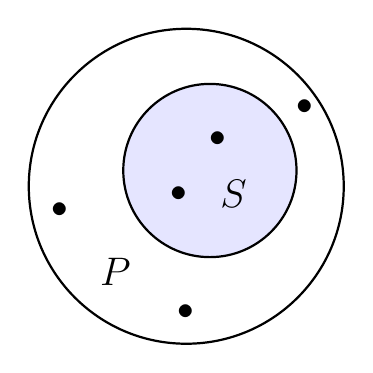
\begin{tikzpicture}
                    \node[circle, draw, thick, minimum size=4cm, label={[xshift=-0.9cm, yshift=-3.4cm]:\Large$P$}] (P) {};
                    \fill[blue!20, opacity=0.5] (0.3,0.2) circle (1.1cm);
                    \node[circle, draw, thick, minimum size=2.2cm, label={[xshift=0.3cm, yshift=-0.3cm]center:\Large$S$}] (S) at (0.3,0.2) {};
                    \node at (0.4, 0.6) {\large$\bullet$}; \node at (-0.1, -0.1) {\large$\bullet$};
                    \node at (1.5, 1) {\large$\bullet$}; \node at (0, -1.6) {\large$\bullet$}; \node at (-1.6, -0.3) {\large$\bullet$};
                \end{tikzpicture}
                {\small Podskupina $S$ želi podpisati sporočilo.}
            \end{figure}
        \end{column}

        \begin{column}{0.55\textwidth}
            \begin{itemize}
                % \item \textbf{Cilj}: Omogočiti poljubni podskupini $S$ znotraj večje skupine $P$, da ustvari en sam podpis.
                \vspace{0.5cm}
                \item \textbf{Ključni lastnosti}:
                \begin{itemize}
                    \item Prilagodljivost%: Podpiše lahko katerakoli podskupina.
                    \item Odgovornost%: Iz podpisa je razvidno, kdo je podpisal.
                \end{itemize}
                \vspace{0.5cm}
                \item \textbf{Analogija}: Fizični podpis pogodbe.
                \vspace{0.5cm}
                \item \textbf{Vprašanje}: Kako bi to dosegli s Schnorrovim podpisom?
            \end{itemize}
        \end{column}
    \end{columns}
    \note[item]{60 s}
    \note[item]{Prvi formalni model, ki ga bomo pogledali, je Večstranski podpis podskupine z odgovornostjo, krajše ASM.}
    \note[item]{Predstavljajmo si, da imamo neko večjo skupino potencialnih podpisnikov, ki jo označimo s $P$. Cilj modela ASM je omogočiti, da katerakoli manjša podskupina $S$ znotraj te skupine ustvari en sam, skupen podpis.}
    \note[item]{Ta model poskuša zadostiti dvema ključnima lastnostma, ki sem jih omenil: \textbf{prilagodljivosti}, saj lahko podpisuje poljubna podskupina, in \textbf{odgovornosti}, saj je iz končnega podpisa vedno razvidno, kdo točno so bili člani skupine $S$.}
    \note[item]{V bistvu deluje natanko tako kot podpisovanje fizične pogodbe – vsi, ki se podpišejo, so jasno navedeni in nosijo odgovornost.}
    \note[item]{Naravno vprašanje je, kako bi takšno shemo zgradili na osnovi Schnorrovega podpisa, ki smo ga pravkar spoznali? Najbolj očitna ideja je, da poskusimo njegove komponente enostavno združiti.}
\end{frame}

\begin{frame}
    \frametitle{Naivna ideja: Združimo komponente}
    % \framesubtitle{Kako bi zgradili večstranski podpis iz Schnorra?}
    \begin{columns}[T]
        \begin{column}{0.5\textwidth}
            \textbf{Individualne komponente}
            \begin{itemize}
                \item Javni ključi: $I_1, I_2, \dots$
                \item Zaveze: $X_1, X_2, \dots$
                \item Odgovori: $y_1, y_2, \dots$
            \end{itemize}
        \end{column}
        \begin{column}{0.5\textwidth}
            \textbf{Agregirane komponente}
            \begin{itemize}
                \item $\tilde{I} = \prod I_i$
                \item $\tilde{X} = \prod X_i$
                \item $\tilde{y} = \sum y_i$
            \end{itemize}
        \end{column}
    \end{columns}
    \vfill
    \begin{center}
        \large
        Izgleda preprosto in elegantno. \textbf{Kje je težava?}
    \end{center}
    \note[item]{30 s}
    \note[item]{Spomnimo se linearne strukture Schnorrovega podpisa. Ta nas naravno vodi do zelo intuitivne ideje za večstranski podpis: enostavno združimo posamezne komponente.}
    \note[item]{Vsak podpisnik prispeva svoj javni ključ $I_i$, svojo zavezo $X_i$ in svoj odgovor $y_i$.}
    \note[item]{Te komponente nato agregiramo: javne ključe in zaveze zmnožimo, odgovore pa seštejemo. Matematično se vse lepo izide in enačba za preverjanje velja.}
    \note[item]{Na prvi pogled je to popolna rešitev – preprosta in učinkovita. Vendar se v tej preprostosti skriva usodna varnostna luknja.}
\end{frame}

\begin{frame}
    \frametitle{Napad: Izničenje ključev}
    % \framesubtitle{Zakaj naivni pristop ne deluje}

    \begin{columns}[T]
        \begin{column}{0.5\textwidth}
            \begin{center}
                \textbf{Poštena podpisnika} \\ Anita \& Bojan
                \vspace{0.5cm}
                Objavita ključa:
                \Large\[ I_A, I_B \]
            \end{center}
        \end{column}

        \begin{column}{0.5\textwidth}
            \begin{center}
                \textbf{Zlonamerni podpisnik} \\ Oskar
                \vspace{0.5cm}
                Počaka in zgradi ključ:
                \Large\[ I_O = (I_A \cdot I_B)^{-1} \cdot g^{s_M} \]
            \end{center}
        \end{column}
    \end{columns}

    \vfill
    \begin{block}{Rezultat: Agregiran javni ključ}
        \large
        \[ \tilde{I} = \underbrace{(I_A \cdot I_B)}_{\text{Anita \& Bojan}} \cdot \underbrace{\left((I_A \cdot I_B)^{-1} \cdot g^{s_M}\right)}_{\text{Oskar}} = g^{s_M} \]
    \end{block}
    % \begin{center}
    %     \large\color{red!80!black}
    %     Agregiran ključ je odvisen samo od Oskarjeve skrivnosti!
    % \end{center}
    \note[item]{60 s}
    \note[item]{Ta varnostna luknja se imenuje \textbf{napad na generiranje ključev} ali izničenje ključev.}
    \note[item]{Poglejmo si, kako deluje. Na levi imamo poštena podpisnika, Anite in Bojana. Normalno objavita svoja javna ključa.}
    \note[item]{Na desni pa imamo zlonamernega Oskarja. On ne ustvari svojega ključa naključno. Počaka, da vidi njuna ključa, in nato svojega zgradi namensko – tako, da bo izničil ostale.}
    \note[item]{In kaj je rezultat? Ko izračunamo agregiran ključ celotne skupine, se, kot vidite v spodnji enačbi, del od Anite in Bojana popolnoma pokrajša z inverznim delom v Oskarjevem ključu.}
    \note[item]{Končni, agregirani ključ je odvisen \textbf{samo} od Oskarjevega zasebnega ključa. To je katastrofa. Oskar lahko sedaj sam podpiše karkoli v imenu celotne skupine.}
\end{frame}

\begin{frame}
    \frametitle{Rešitev: Dokazi znanja brez razkritja znanja}
    % \framesubtitle{Rešitev napada na generiranje ključev}

        % \item Dokaz, da nekaj vemo, ne da bi razkrili, kaj vemo.
        % \item Preprečujejo, da bi napadalec ponaredil javni ključ.
    \begin{itemize}
        \item Vsak podpisnik (tudi Oskar) mora dokazati, da pozna svoj zasebni ključ.
        \item To prepreči napad na generiranje ključev.
        \item V praksi je to standarden Schnorrov podpis, ki dokazuje lastništvo ključa.
    \end{itemize}
    \vspace{1cm}
    \begin{figure}
        \begin{subfigure}{0.28\textwidth}
            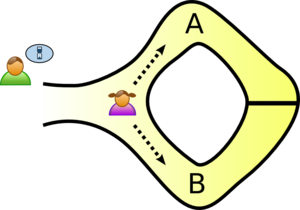
\includegraphics[width=\textwidth]{images/zkp1.png}
        \end{subfigure}
        \hspace{0.25cm}
        \begin{subfigure}{0.25\textwidth}
            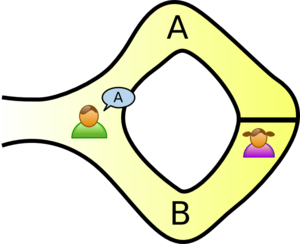
\includegraphics[width=\textwidth]{images/zkp2.png}
        \end{subfigure}
        \hspace{0.25cm}
        \begin{subfigure}{0.25\textwidth}
            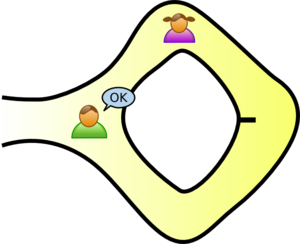
\includegraphics[width=\textwidth]{images/zkp3.png}
        \end{subfigure}
    \end{figure}
    \note[item]{90 s}
    \note[item]{Torej, kako rešimo problem Oskarjevega napada? Rešitev je uporaba dokazov znanja.}
    \note[item]{Od vsakega podpisnika, vključno z Oskarjem, zahtevamo, da ob objavi svojega javnega ključa $I_i$ predloži tudi kriptografski dokaz, da dejansko pozna pripadajoči zasebni ključ $s_i$.}
    \note[item]{S tem Oskar ne more več zgraditi svojega ključa iz ključev drugih, saj zanj ne bi poznal ustreznega zasebnega ključa in posledično ne bi mogel ustvariti veljavnega dokaza. Napad je s tem preprečen.}
    \note[item]{Koncept, ki to omogoča, se imenuje dokaz znanja brez razkritja znanja. Idejo najlažje razumemo z analogijo o Ali Babini jami. Anita želi Bojanu dokazati, da pozna skrivno geslo za vrata, ne da bi mu geslo sama povedala. Bojan jo zato večkrat postavi pred izziv, in po dovolj ponovitvah je prepričan v njeno znanje, čeprav skrivnosti ni nikoli izvedel.}
    \note[item]{V naši shemi vlogo tega dokaza odigra kar en standarden Schnorrov podpis. To pa, kot bomo videli, v shemo vnese dodatno kompleksnost in neučinkovitost, ki jo moramo nasloviti.}
\end{frame}

\begin{frame}[fragile]
    \frametitle{Nadgradnja: Merklova drevesa}
    % \framesubtitle{Učinkovita zaveza skupini}

    \begin{center}
        \large\color{red!80!black}
        \textbf{Problem:} Preverjanje $L$ dokazov znanja je neučinkovito.
    \end{center}

    \begin{figure}
        \centering
        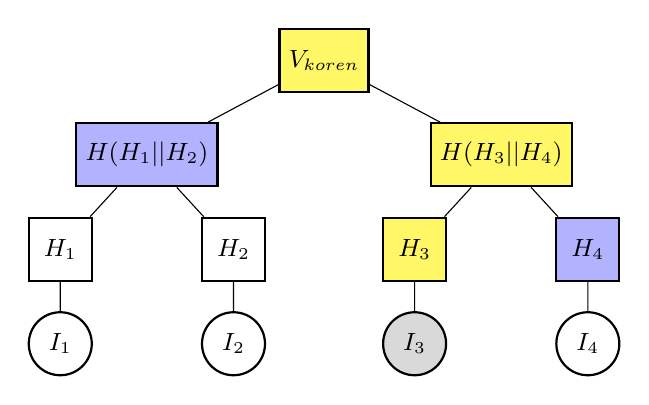
\begin{tikzpicture}[
            level distance=1.2cm,
            level 1/.style={sibling distance=4.5cm},
            level 2/.style={sibling distance=2.2cm},
            treenode/.style={rectangle, draw, thick, minimum size=0.8cm, font=\small},
            leaf_node/.style={circle, draw, thick, minimum size=0.8cm, font=\small}, % New style for leaf nodes
            path_node/.style={treenode, fill=yellow!60},
            sibling_node/.style={treenode, fill=blue!30},
            our_key/.style={leaf_node, fill=gray!30, text=black} % Highlight our key
        ]
            % The tree structure
            \node[path_node] (root) {$V_{koren}$}
                child { node[sibling_node] (h12) {$H(H_1||H_2)$}
                    child { node[treenode] (h1) {$H_1$} child {node[leaf_node]{$I_1$}} }
                    child { node[treenode] (h2) {$H_2$} child {node[leaf_node]{$I_2$}} }
                }
                child { node[path_node] (h34) {$H(H_3||H_4)$}
                    child { node[path_node] (h3) {$H_3$} child {node[our_key]{$I_3$}} }
                    child { node[sibling_node] (h4) {$H_4$} child {node[leaf_node]{$I_4$}} }
                };
        \end{tikzpicture}

        \small \textbf{Rešitev:} Dokazilo o pripadnosti ključa $I_3$ z \color{blue!60} overjevalno potjo.
    \end{figure}
    \begin{center}
        \large\color{blue!60!black}
        Velikost poti je le $\log(L)$.
    \end{center}
    \note[item]{60 s}
    \note[item]{Rešitev z dokazi znanja reši varnostni problem, a ustvari novega: neučinkovitost. Če bi morali preverjati dokaz za vsakega od stotih podpisnikov, bi sistem postal neuporaben.}
    \note[item]{To rešimo z Merklovim drevesom. Namesto da hranimo vse ključe, jih zgoščamo v drevesno strukturo, dokler na vrhu ne dobimo ene same, kratke vrednosti – korena drevesa. Ta koren služi kot kriptografska zaveza celotni skupini.}
    \note[item]{Posamezen podpisnik, na primer za ključ $I_3$, zdaj ne rabi več dokazovati vsega. Dokazati mora le, da je njegov ključ del drevesa, ki ima ta javni koren.}
    \note[item]{To stori s pomočjo \textbf{overjevalne poti}. Ta pot vsebuje samo sosednja vozlišča na poti od njegovega lista do korena – to so elementi, obarvani modro. Preverjevalec vzame $I_3$, ga zgosti, združi z modrim $H_4$, ponovno zgosti, združi z modrim $H(H_1||H_2)$ in še zadnjič zgosti. Če se rezultat ujema z javnim korenom, je dokaz veljaven.}
    \note[item]{Ključno je, da velikost te poti raste le logaritemsko. Za tisoč podpisnikov potrebujemo le okoli 10 zgoščenih vrednosti, kar ohranja sistem izjemno učinkovit.}
\end{frame}

\begin{frame}
    \frametitle{Protokol ASM: Priprava}
    % \framesubtitle{Enkratni postopek za vzpostavitev skupine}

    \begin{columns}[T]
        \begin{column}{0.33\textwidth}
            \centering
            \tikz\node[circle,draw,thick,minimum size=0.9cm] {\Large 1}; 
            \vspace{0.3cm}
            
            \textbf{Generiranje ključev}
            \begin{itemize}
                \item Vsak član ustvari svoj par ključev $(s_i, I_i)$.
            \end{itemize}
        \end{column}

        \begin{column}{0.33\textwidth}
            \centering
            \tikz\node[circle,draw,thick,minimum size=0.9cm] {\Large 2};
            \vspace{0.3cm}
            
            \textbf{Dokaz znanja}
            \begin{itemize}
                \item Vsak dokaže lastništvo ključa (preprečitev napada).
            \end{itemize}
        \end{column}

        \begin{column}{0.33\textwidth}
            \centering
            \tikz\node[circle,draw,thick,minimum size=0.9cm] {\Large 3};
            \vspace{0.3cm}
            
            \textbf{Zaveza skupini}
            \begin{itemize}
                \item Zgradi se Merklovo drevo za učinkovitost.
            \end{itemize}
        \end{column}
    \end{columns}

    \vfill
    \begin{center}
        \large
        Po končani pripravi je skupina nared za podpisovanje.
    \end{center}
    \note[item]{30 s}
    \note[item]{Poglejmo si torej celoten protokol ASM. Začne se z \textbf{enkratno pripravo} za vzpostavitev skupine.}
    \note[item]{Najprej vsak potencialni član ustvari svoj par Schnorrovih ključev.}
    \note[item]{Nato, da preprečimo napad izničenja, vsak objavi dokaz, da resnično pozna svoj zasebni ključ.}
    \note[item]{In končno, za učinkovitost, se vsi javni ključi združijo v eno Merklovo drevo z enim samim korenom.}
    \note[item]{Ta postopek se izvede samo enkrat. Ko je končan, je skupina pripravljena na podpisovanje poljubnega števila dokumentov.}
\end{frame}

\begin{frame}
    \frametitle{Protokol ASM: Podpisovanje}
    % \framesubtitle{Interaktivni protokol v 3 krogih}
    \begin{figure}
        \centering
        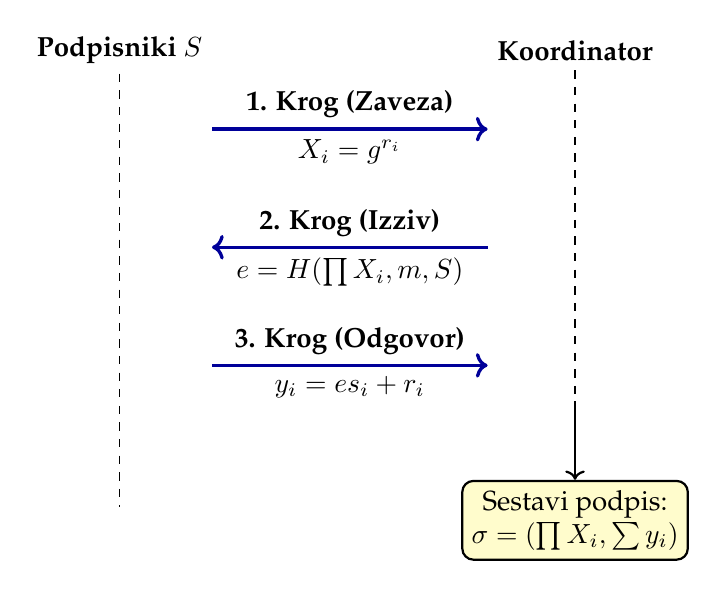
\begin{tikzpicture}[
            node distance=0.8cm and 3.5cm,
            participant/.style={align=center, font=\bfseries},
        ]
            \node[participant] (signers) {Podpisniki $S$};
            \node[participant, right=of signers] (coord) {Koordinator};
            
            \draw[dashed] (signers.south) -- ++(0,-5.5);
            \draw[dashed] (coord.south) -- ++(0,-5.5);
            
            \draw[->, very thick, blue!60!black] ([yshift=-1cm]signers.east) -- ([yshift=-1cm]coord.west)
                node[midway, above, black] {\textbf{1. Krog (Zaveza)}}
                node[midway, below, black] {$X_i = g^{r_i}$};
                
            \draw[<-, very thick, blue!60!black] ([yshift=-2.5cm]signers.east) -- ([yshift=-2.5cm]coord.west)
                node[midway, above, black] {\textbf{2. Krog (Izziv)}}
                node[midway, below, black, align=center] {$e = H(\prod X_i, m, S)$};
                
            \draw[->, very thick, blue!60!black] ([yshift=-4cm]signers.east) -- ([yshift=-4cm]coord.west)
                node[midway, above, black] {\textbf{3. Krog (Odgovor)}}
                node[midway, below, black] {$y_i = es_i + r_i$};
                
            \node[draw, thick, fill=yellow!20, rounded corners, below=0.2cm of coord, yshift=-5cm, align=center] (assembly) {Sestavi podpis:\\$\sigma = (\prod X_i, \sum y_i)$};
            \draw[->, thick] ([yshift=-4.2cm]coord.south) -- (assembly.north);

        \end{tikzpicture}
    \end{figure}
    \note[item]{60 s}
    \note[item]{Sedaj pa k samemu podpisovanju. Ko želi podskupina podpisati sporočilo, to stori z interaktivnim protokolom v treh krogih.}
    \note[item]{V \textbf{prvem krogu} vsak podpisnik pošlje svojo zavezo $X_i$ koordinatorju.}
    \note[item]{V \textbf{drugem krogu} koordinator združi vse prejete zaveze, izračuna en sam skupni izziv $e$ in ga pošlje nazaj vsem podpisnikom.}
    \note[item]{V \textbf{tretjem krogu} vsak podpisnik uporabi ta izziv, da izračuna svoj delni podpis $y_i$, in ga pošlje koordinatorju.}
    \note[item]{Koordinator na koncu preprosto sešteje vse delne podpise in sestavi končni večstranski podpis.}
    \note[item]{In to je ključni kompromis sheme ASM: je varna, je prilagodljiva in zagotavlja odgovornost. Vendar pa so ti trije krogi komunikacije v praksi počasni in predstavljajo glavno pomanjkljivost te sheme.}
\end{frame}

\begin{frame}
    \frametitle{Varnost ASM}
    % \framesubtitle{Dokaz z redukcijo}
    \begin{itemize}
        \item Shema je \textbf{dokazljivo varna} v modelu slučajnega oraklja.
        \vspace{0.5cm}
        \item Varnost se z \textbf{redukcijo} prevede na \textbf{težavnost problema diskretnega logaritma}.
        \vspace{0.5cm}
        \item Ključno orodje v dokazu je \textbf{lema o razcepu} (angl. \textit{Forking Lemma}).
        \begin{itemize}
            \item Če napadalec lahko ponaredi podpis, ga lahko z "previjanjem nazaj" prisilimo, da z istimi podatki in drugačnim izzivom ustvari še en ponaredek.
            \item Iz dveh ponaredkov lahko izračunamo zasebni ključ in tako rešimo problem diskretnega logaritma.
        \end{itemize}
        \vspace{0.5cm}
        \item \textbf{Zaključek}: Shema je varna, prilagodljiva in zagotavlja odgovornost, a trije krogi komunikacije so lahko prepočasni.
    \end{itemize}
    % \note[item]{60 s}
    % \note[item]{The ASM scheme is provably secure in the Random Oracle Model.}
    % \note[item]{Its security reduces to the hardness of the Discrete Logarithm Problem.}
    % \note[item]{The proof relies on the Forking Lemma: if an attacker can forge a signature, we can use that attacker as a tool to solve the underlying hard problem.}
    % \note[item]{Verdict: ASM is secure, flexible, and provides full accountability.}
    % \note[item]{But... three rounds of communication can be too slow for many real-world applications.}
    \note[item]{60 s}
    \note[item]{Po sestavi tako kompleksnega protokola se moramo vprašati: kako smo lahko prepričani, da je varen? Odgovor je v 'dokazu z redukcijo'.}
    \note[item]{Varnost sheme ASM je formalno dokazana in je enakovredna težavnosti enega temeljnih matematičnih problemov: problema diskretnega logaritma, za katerega verjamemo, da ga noben učinkovit računalnik ne more rešiti.}
    \note[item]{ Logika dokaza je naslednja: Predpostavimo, da obstaja nek napadalec, ki lahko prelomi našo shemo in ustvari ponarejen podpis.}
    \note[item]{Mi nato zgradimo 'stroj', ki temelji na orodju, imenovanem \textbf{lema o razcepu}. Ta lema nam omogoča, da napadalca 'previjemo nazaj' in ga pretentamo, da z istimi začetnimi podatki ustvari še \textit{drug} ponaredek.}
    \note[item]{Z dvema različnima ponaredkoma lahko nato z nekaj algebre izračunamo zasebni ključ, kar pomeni, da smo rešili problem diskretnega logaritma.}
    \note[item]{Tukaj pridemo do protislovja. Če naš napadalec obstaja, lahko rešimo nerešljiv problem. Edini logičen sklep je, da naša začetna predpostavka ne drži: \textbf{tak napadalec ne more obstajati}, in zato je shema ASM varna.}
    \note[item]{Torej, končna sodba o ASM je: je varna, prilagodljiva in zagotavlja odgovornost. Njena edina resnična slabost pa ostajajo trije počasni krogi komunikacije.}
\end{frame}

\begin{frame}
    \frametitle{Moderne zahteve}
    % \framesubtitle{Od odgovornosti k učinkovitosti in zasebnosti}
    \begin{columns}[T]
        \begin{column}{0.5\textwidth}
            \begin{block}{Omejitve sheme ASM}
                \begin{itemize}
                    \item \textbf{Počasnost:} 3 krogi komunikacije so prepočasni.% za aplikacije, kot so kriptovalute.
                    \item \textbf{Pomanjkanje zasebnosti:} Polna odgovornost ni vedno zaželena.
                \end{itemize}
            \end{block}
        \end{column}

        \begin{column}{0.5\textwidth}
            \begin{block}{Novi cilji}
                \begin{itemize}
                    \item \textbf{Hitrost:} Doseči 2-krožno shemo.
                    \item \textbf{Zasebnost:} Omogočiti zamenljivost s standardnim podpisom in skriti podpisnike.
                \end{itemize}
            \end{block}
        \end{column}
    \end{columns}

    \vfill
    \Huge\centering$\Downarrow$\par
    \vfill

    \large Menjava \textbf{odgovornosti} za večjo \textbf{učinkovitost} in \textbf{zasebnost}.
    \note[item]{30 s}
    \note[item]{Videli smo, da je protokol ASM varen in zagotavlja odgovornost. Zakaj se je torej razvoj nadaljeval? Odgovor leži v modernih zahtevah, ki jih narekujejo aplikacije, kot so kriptovalute.}
    \note[item]{Shema ASM ima dve ključni omejitvi. Prvič, njeni trije krogi komunikacije so preprosto prepočasni. Drugič, polna odgovornost, kjer je vsak podpisnik javno viden, ni vedno zaželena – včasih je bolj pomembna zasebnost.}
    \note[item]{To je vodilo do novih ciljev: razviti bistveno hitrejšo, 2-krožno shemo, ki hkrati poveča zasebnost podpisnikov.}
    \note[item]{Da bi to dosegli, je bil potreben temeljni kompromis, ki je osrednja točka druge polovice mojega dela: zamenjati odgovornost in prilagodljivost za bistveno večjo učinkovitost in zasebnost. To nas pripelje do sodobne rešitve: protokola MuSig2.}
\end{frame}

\begin{frame}
    \frametitle{MuSig2}
    % \framesubtitle{Učinkovitost in zasebnost v praksi}
    \begin{columns}[T]
        \begin{column}{0.45\textwidth}
            \centering
            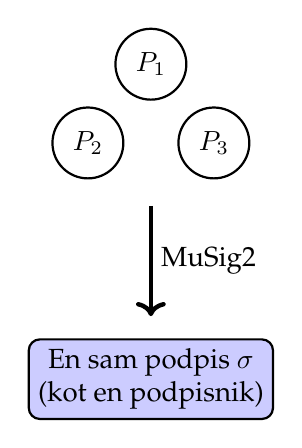
\begin{tikzpicture}[
                signer/.style={circle, draw, thick, minimum size=0.9cm},
                final_box/.style={rectangle, draw, thick, rounded corners, fill=blue!20, align=center, minimum width=2.8cm}
            ]
                \node[signer] (s1) at (0, 2.5) {$P_1$};
                \node[signer] (s2) at (-0.8, 1.5) {$P_2$};
                \node[signer] (s3) at (0.8, 1.5) {$P_3$};

                \draw[->, thick, double distance=0pt] (0, 0.7) -- (0, -0.7) node[midway, right] {MuSig2};

                \node[final_box] at (0, -1.5) {En sam podpis $\sigma$ \\ (kot en podpisnik)};
            \end{tikzpicture}
            % \captionof{figure}{\small Več podpisnikov $\rightarrow$ en podpis.}
        \end{column}
        \begin{column}{0.55\textwidth}
            \begin{itemize}
                \item \textbf{Hitrost:} Zahteva samo \textbf{dva kroga} komunikacije.
                \item \textbf{Učinkovitost:} Uporablja \textbf{agregacijo ključev}.
                \item \textbf{Združljivost:} Rezultat je \textbf{standarden Schnorrov podpis}.
                \item \textbf{Zasebnost:} Podpis je nerazločljiv od podpisa posameznika.
            \end{itemize}
        \end{column}
    \end{columns}
    \note[item]{60 s}
    \note[item]{Ko smo se odpovedali odgovornosti, kaj smo pridobili v zameno? Dobili smo sodoben in visoko učinkovit protokol, imenovan MuSig2.}
    \note[item]{Osrednji koncept MuSig2 je izjemno močan. Omogoča, da se skupina več podpisnikov združi in ustvari en sam podpis, ki je za zunanji svet videti natanko tako kot standarden podpis ene same osebe z enim samim ključem. Preverjevalec ne more ugotoviti razlike.}
    \note[item]{Ta pristop prinaša štiri ključne prednosti:}
    \note[item]{Prvič, \textbf{hitrost}: Dosegli smo cilj in zmanjšali komunikacijo na samo dva kroga.}
    \note[item]{Drugič, \textbf{učinkovitost}: To je mogoče zaradi agregacije ključev, kjer se več javnih ključev matematično združi v enega samega.}
    \note[item]{Tretjič, \textbf{združljivost}: Ker je rezultat standarden Schnorrov podpis, ga lahko uporabimo v kateremkoli obstoječem sistemu, ki že razume Schnorra. Je direktna zamenjava.}
    \note[item]{In končno, \textbf{zasebnost}: Ker podpisa ni mogoče ločiti od navadnega, preverjevalec ne ve – in mu ni treba vedeti – kdo ali koliko oseb je sodelovalo pri podpisu. To močno poveča zasebnost.}
\end{frame}

\begin{frame}
    \frametitle{Kako deluje MuSig2?}
    % \framesubtitle{Varna agregacija in podpisovanje v 2 krogih}
    \begin{columns}[T]
        \begin{column}{0.5\textwidth}
            \begin{block}{1. Varna agregacija ključev}
                Napad na generiranje ključev je preprečen s koeficienti $c_i$, ki so odvisne od \textbf{vseh} ključev v skupini.
            \end{block}
            \centering
            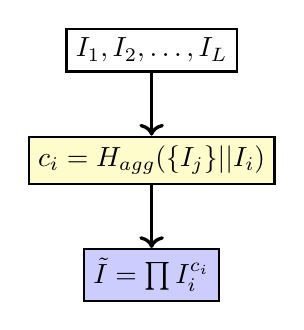
\begin{tikzpicture}[node distance=0.8cm]
                \node (keys) [draw, thick, align=center] {$I_1, I_2, \dots, I_L$};
                \node (hash) [draw, thick, fill=yellow!20, below=of keys] {$c_i = H_{agg}(\{I_j\} || I_i)$};
                \node (agg_key) [draw, thick, fill=blue!20, below=of hash] {$\tilde{I} = \prod I_i^{c_i}$};
                \draw[->, very thick] (keys) -- (hash);
                \draw[->, very thick] (hash) -- (agg_key);
            \end{tikzpicture}
        \end{column}

        \begin{column}{0.5\textwidth}
            \begin{block}{2. Podpisovanje v 2 krogih}
                \centering
                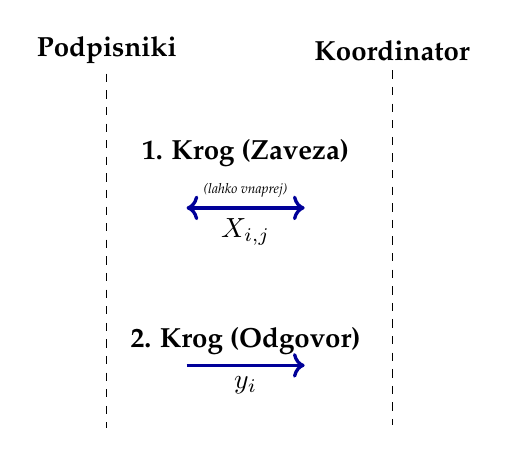
\begin{tikzpicture}[
                    node distance=0.8cm and 1.5cm,
                    participant/.style={align=center, font=\bfseries},
                ]
                    \node[participant] (signers) {Podpisniki};
                    \node[participant, right=of signers] (coord) {Koordinator};
                    
                    \draw[dashed] (signers.south) -- ++(0,-4.5);
                    \draw[dashed] (coord.south) -- ++(0,-4.5);
                    
                    \draw[<->, very thick, blue!60!black] ([yshift=-2cm]signers.east) -- ([yshift=-2cm]coord.west)
                        node[midway, above, black, align=center] {\textbf{1. Krog (Zaveza)} \\ \tiny\itshape(lahko vnaprej)}
                        node[midway, below, black] {$X_{i, j}$};

                    \draw[->, very thick, blue!60!black] ([yshift=-4cm]signers.east) -- ([yshift=-4cm]coord.west)
                        node[midway, above, black] {\textbf{2. Krog (Odgovor)}}
                        node[midway, below, black] {$y_i$};
                \end{tikzpicture}
            \end{block}
        \end{column}
    \end{columns}

    \note[item]{90 s}
    \note[item]{Poglejmo si dve ključni inovaciji, ki omogočata delovanje MuSig2.}
    \note[item]{Prva je \textbf{varna agregacija ključev}. Kako MuSig2 prepreči napad izničenja? Namesto da samo zmnoži ključe, izračuna uteženo vsoto. Ključno je, da je utež $c_i$ za vsak ključ odvisna od \textit{vseh} ključev v skupini. S tem Oskar ne more več zgraditi svojega ključa neodvisno, saj je njegov koeficient odvisen od ključev Anite in Bojana, in obratno. Ta medsebojna odvisnost prepreči napad.}
    \note[item]{Druga inovacija je izjemno učinkovit \textbf{protokol podpisovanja v dveh krogih}.}
    \note[item]{\textbf{Prvi krog} je izmenjava zavez oziroma `nonce-ov`. Bistvena prednost je, da se ta krog lahko izvede \textit{vnaprej}, preden je sporočilo za podpis sploh znano. Podpisniki si lahko te zaveze izmenjajo kadarkoli.}
    \note[item]{\textbf{Drugi krog} se zgodi, ko je sporočilo znano. Takrat vsak podpisnik izračuna in pošlje svoj delni podpis.}
    \note[item]{Ker se prvi krog lahko opravi vnaprej, je v praksi podpisovanje skoraj takojšnje – zahteva le en krog komunikacije, ko je treba nekaj podpisati. To je tisto, kar naredi MuSig2 tako hiter.}
\end{frame}

\begin{frame}
    \frametitle{Empirična analiza}
    % \framesubtitle{Odgovornost ali učinkovitost v praksi?}
    \begin{block}{Primerjane sheme}
        \begin{columns}[T,totalwidth=\textwidth] % Use full width for better spacing
            \begin{column}{0.33\textwidth}
                \textbf{1. Osnova}
                \begin{itemize}
                    \item Schnorr
                \end{itemize}
            \end{column}
            \begin{column}{0.33\textwidth}
                \textbf{2. Odgovornost}
                \begin{itemize}
                    \item Shema ASM
                \end{itemize}
            \end{column}
            \begin{column}{0.33\textwidth}
                \textbf{3. Učinkovitost}
                \begin{itemize}
                    \item MuSig2
                \end{itemize}
            \end{column}
        \end{columns}
    \end{block}

    \vfill

    \begin{block}{Merjeni parametri}
        \centering
        \large
        Generiranje ključev \quad$\cdot$\quad Podpisovanje \quad$\cdot$\quad Preverjanje
        \vspace{0.5cm}
        \large\textit{...vse v odvisnosti od števila podpisnikov.}
    \end{block}
    \note[item]{30 s}
    \note[item]{Da bi teoretične prednosti in slabosti teh shem preveril tudi v praksi, sem izvedel empirično analizo učinkovitosti.}
    \note[item]{ Primerjal sem tri ključne pristope: prvič, osnovni pristop z nizanjem posameznih Schnorrovih podpisov. Drugič, shemo, osredotočeno na odgovornost, torej ASM. In tretjič, shemo, osredotočeno na učinkovitost, MuSig2.}
    \note[item]{ Za vsak pristop sem meril časovno zahtevnost treh glavnih operacij: generiranja ključev, podpisovanja in preverjanja.}
    \note[item]{Vse meritve so bile izvedene v odvisnosti od naraščajočega števila podpisnikov, da bi videli, kako posamezna shema skalira. Poglejmo si rezultate.}
\end{frame}

\begin{frame}
    \frametitle{Rezultati: Generiranje ključev in Podpisovanje}
    \begin{columns}[T]
        \begin{column}{0.5\textwidth}
            \centering
            \textbf{1. Generiranje ključev}
            
\includegraphics[width=\linewidth]{images/benchmark_KeyGeneration.pdf}
            
            % \begin{block}{Ugotovitev}
            \begin{block}
                \small % Use a smaller font for the finding
                \textbf{ASM je najpočasnejši} zaradi kompleksne priprave (dokazi znanja, Merklovo drevo), ki se izvede le enkrat. 
            \end{block}
        \end{column}

        \begin{column}{0.5\textwidth}
            \centering
            \textbf{2. Podpisovanje}
            
\includegraphics[width=\linewidth]{images/benchmark_Signing.pdf}
            
            % \begin{block}{Ugotovitev}
            \begin{block}
                \small
                MuSig2 zahteva več računskega dela, a je v praksi \textbf{bistveno hitrejši} zaradi manj komunikacije (2 vs. 3 krogi). 
            \end{block}
        \end{column}
    \end{columns}
    \note[item]{60 s}
    \note[item]{Poglejmo si prve rezultate meritev. Na tej prosojnici sta grafa za čas generiranja ključev in čas podpisovanja. Pomembno je poudariti, da grafi prikazujejo samo čas računanja in ne vključujejo zakasnitev omrežja.}
    \note[item]{ Pri \textbf{generiranju ključev}, kot je pričakovano, je shema ASM bistveno počasnejša.  To je posledica kompleksnega postopka priprave, ki vključuje dokaze znanja in gradnjo Merklovega drevesa.  Navadni Schnorr in MuSig2 sta mnogo hitrejša. }
    \note[item]{ Pri \textbf{podpisovanju} pa graf pokaže nekaj zanimivega: MuSig2 je v smislu samega računanja najpočasnejši.  To je zaradi bolj zapletenih korakov pri agregaciji.}
    \note[item]{Vendar pa je tu ključnega pomena opozorilo: ta graf zanemarja čas komunikacije. V realnem svetu dejstvo, da MuSig2 potrebuje samo dva kroga komunikacije v primerjavi s tremi pri ASM, pomeni, da je v praksi \textit{bistveno} hitrejši. Računski dodatek je zanemarljiv v primerjavi s prihrankom pri komunikaciji. }
\end{frame}

\begin{frame}
    \frametitle{Rezultati: Preverjanje}
    % \framesubtitle{Glavna prednost večstranskih podpisov}
    \begin{figure}
        \centering
        
\includegraphics[width=0.85\textwidth]{images/benchmark_Verification.pdf}
    \end{figure}

    \begin{columns}[T,totalwidth=\textwidth]
        \begin{column}{0.33\textwidth}
            \centering
            \color{orange!80!black}\large\bfseries 1. Schnorr
            \rmfamily\normalsize
            \begin{itemize}
                \item Čas narašča \textbf{linearno}.
                \item Ni skalabilno.
            \end{itemize}
        \end{column}
        
        \begin{column}{0.33\textwidth}
            \centering
            \color{green!50!black}\large\bfseries 2. ASM
            \rmfamily\normalsize
            \begin{itemize}
                \item Rast je \textbf{zelo počasna}.
                \item Učinkovito.
            \end{itemize}
        \end{column}
        
        \begin{column}{0.33\textwidth}
            \centering
            \color{blue!60!black}\large\bfseries 3. MuSig2
            \rmfamily\normalsize
            \begin{itemize}
                \item Čas je \textbf{konstanten}.
                \item Idealno.
            \end{itemize}
        \end{column}
    \end{columns}
    \note[item]{60 s}
    \note[item]{In sedaj pridemo do najpomembnejšega rezultata, ki prikaže glavno prednost večstranskih podpisov: čas preverjanja.}
    \note[item]{Ta graf pove celotno zgodbo. Poglejmo si najprej zgornjo črto.}
    \note[item]{Pri navadnem nizanju Schnorrovih podpisov čas preverjanja narašča \textbf{linearno}. To za mnoge aplikacije ni skalabilno.}
    \note[item]{Shema ASM je ogromen napredek. Zaradi Merklovih dreves čas preverjanja narašča zelo počasi – logaritmično. To je že zelo učinkovito.}
    \note[item]{A idealna rešitev je MuSig2. Čas preverjanja je \textbf{konstanten}. Traja enako dolgo, ne glede na to, ali je podpisnik en ali jih je dvesto. To je zlati standard učinkovitosti.}
    \note[item]{Ta graf torej popolnoma oriše kompromis: da dosežemo ta neverjeten, konstanten čas preverjanja, se je MuSig2 moral odpovedati odgovornosti, ki jo ponuja ASM.}
\end{frame}

\begin{frame}
    \frametitle{Primerjava shem}
    % \framesubtitle{Pregled ključnih lastnosti}
    \centering
    \renewcommand{\arraystretch}{1.5} % Your original row spacing
    \footnotesize % Your original font size

    \begin{tabular}{|l|c|c|c|}
        \hline
        \textbf{Lastnost} & \textbf{Schnorr} & \textbf{ASM} & \textbf{MuSig2} \\ \hline
        Čas preverjanja   & \cellcolor{bad}Linearen      & \cellcolor{ok}Konstanten* & \cellcolor{good}Konstanten \\ \hline
        Odgovornost       & \cellcolor{good}Popolna       & \cellcolor{good}Popolna        & \cellcolor{bad}Brez \\ \hline
        Prilagodljivost   & \cellcolor{good}Popolna       & \cellcolor{good}Popolna        & \cellcolor{bad}Brez (cela skupina) \\ \hline
        Komunikacija      & \cellcolor{good}0 krogov      & \cellcolor{bad}3 krogi         & \cellcolor{ok}2 kroga \\ \hline
        Zasebnost         & \cellcolor{bad}Brez           & \cellcolor{bad}Brez            & \cellcolor{good}Popolna \\ \hline
    \end{tabular}
    \note[item]{60 s}
    \note[item]{Ta tabela združi vse naše ugotovitve in jasno prikaže kompromise med shemami.}
    \note[item]{Poglejmo si ključne točke. Pri \textbf{času preverjanja}, ki je glavna motivacija za večstranske podpise, vidimo jasno zgodbo: navadno nizanje je neskalabilno. ASM je ogromen napredek. MuSig2 pa doseže teoretični ideal: konstanten čas preverjanja.}
    \note[item]{Kakšna pa je cena te učinkovitosti? Poglejmo \textbf{odgovornost} in \textbf{prilagodljivost}. Tu sta osnovni pristop in ASM popolna – natančno vemo, kdo je podpisal. MuSig2 teh lastnosti nima.}
    \note[item]{Nasprotje pa velja za \textbf{zasebnost}. Kjer ASM ne ponuja nobene, MuSig2 ponuja popolno zasebnost, saj je podpis nerazločljiv od navadnega.}
    \note[item]{Tabela torej jasno pokaže, da ne obstaja ena sama 'najboljša' rešitev za vse primere. Izbira je vedno kompromis, kar nas pripelje do končnega zaključka.}
\end{frame}

\begin{frame}
    \frametitle{Kompromis}
    % \framesubtitle{Odgovornost ali učinkovitost?}
    % Izbira sheme je odvisna od zahtev aplikacije.
    % \vspace{1cm}
    %
    \begin{columns}[T]
        \begin{column}{0.5\textwidth}
            \begin{beamercolorbox}[sep=0.3cm,center]{block title}
                \textbf{Izberi ASM, ko ...}
            \end{beamercolorbox}
            \begin{beamercolorbox}[sep=0.3cm,ht=5cm]{block body}
                \begin{itemize}
                    \item ... je \textbf{odgovornost} ključna (mora se vedeti, kdo je podpisal).
                    \item ... je \textbf{prilagodljivost} pomembna (podpisujejo lahko poljubne podskupine).
                    \item ... so 3 krogi komunikacije sprejemljivi.
                \end{itemize}
            \end{beamercolorbox}
        \end{column}
        \begin{column}{0.5\textwidth}
            \begin{beamercolorbox}[sep=0.3cm,center]{block title}
                \textbf{Izberi MuSig2, ko ...}
            \end{beamercolorbox}
            \begin{beamercolorbox}[sep=0.3cm,ht=5cm]{block body}
                \begin{itemize}
                    \item ... je \textbf{učinkovitost preverjanja} najpomembnejša.
                    \item ... je zaželena \textbf{zasebnost} podpisnikov.
                    \item ... potrebujete združljivost z obstoječo Schnorr infrastrukturo (npr. Bitcoin).
                \end{itemize}
            \end{beamercolorbox}
        \end{column}
    \end{columns}
    \note[item]{60 s}
    \note[item]{Po vsem tem se postavlja vprašanje: katera shema je boljša? Odgovor je, da je odvisno od aplikacije.}
    \note[item]{Shemo \textbf{ASM} boste izbrali takrat, kadar sta na prvem mestu odgovornost in prilagodljivost. Torej, kadar morate natančno vedeti, kdo je podpisal, in kadar morajo poljubne podskupine imeti možnost podpisovanja. To je prava izbira za digitalne pogodbe ali formalna glasovanja, kjer je sprejemljivo, da je komunikacija počasnejša.}
    \note[item]{Po drugi strani boste izbrali \textbf{MuSig2}, kadar sta najpomembnejši absolutna učinkovitost in zasebnost. Ko potrebujete najhitrejše možno preverjanje in želite, da podpisniki ostanejo anonimni, je MuSig2 idealen. Zaradi združljivosti s standardnim Schnorrom je to tudi očitna izbira za sisteme, kot je Bitcoin.}
\end{frame}

\begin{frame}
    \frametitle{Prihodnje delo}
    % \framesubtitle{Odgovornost ali učinkovitost?}
    \begin{itemize}
        \item \textbf{Podrobnejša empirična analiza}
        \begin{itemize}
            \item Izvedba meritev v realnem omrežju, kjer se upošteva dejanski čas komunikacije.
            \item Analiza optimizacij, kot je shranjevanje Merklovega drevesa med zaporednimi podpisi pri ASM.
        \end{itemize}
        \vspace{1cm}
        \item \textbf{Post-kvantni večstranski podpisi}
        \begin{itemize}
            \item Schnorr in sorodne sheme niso varne pred napadi kvantnih računalnikov.
            \item Raziskave so usmerjene v sheme, ki temeljijo na problemih na rešetkah (angl. \textit{lattice problems}).
            \item Primer: \textbf{MuSig-L} kot post-kvantna različica MuSig2.
        \end{itemize}
    \end{itemize}
    \note[item]{60 s}
    \note[item]{Za konec, kam bi lahko to delo vodilo naprej? Vidim dve glavni smeri.}
    \note[item]{Prva in najpomembnejša je \textbf{post-kvantna varnost}. Vse sheme, ki smo jih danes obravnavali, temeljijo na problemu diskretnega logaritma, ki ga lahko reši dovolj močan kvantni računalnik. Prihodnost večstranskih podpisov je zato v shemah, ki temeljijo na drugačnih, kvantno odpornih problemih, kot so problemi na mrežah. Zanimiv primer je MuSig-L, ki poskuša biti post-kvantna alternativa MuSig2.}
    \note[item]{Druga smer je \textbf{bolj poglobljena empirična analiza}. Moje meritve so se osredotočile na računsko zahtevnost. Naslednji logičen korak bi bil implementacija v realnem omrežju, da bi natančno izmerili vpliv komunikacije in zakasnitev. Prav tako bi bilo zanimivo analizirati učinek praktičnih optimizacij, na primer, kako shranjevanje Merklovega drevesa vpliva na hitrost zaporednih podpisov znotraj iste skupine pri shemi ASM.}
\end{frame}

\begin{frame}
    \frametitle{Zaključek}
    \framesubtitle{Odgovornost ali učinkovitost?}

    \begin{beamercolorbox}[sep=0.3cm,center,rounded=true,shadow=true]{block title}
        Ključna prednost: \textbf{Učinkovito preverjanje}, neodvisno od števila podpisnikov.
    \end{beamercolorbox}

    \vspace{1cm}

    \begin{columns}[T]
        \begin{column}{0.5\textwidth}
            \centering
            \large\textbf{Pristop 1: ASM}
            \begin{itemize}
                \item \color{good!50!black}\textbf{+ Odgovornost}
                \item \color{good!50!black}\textbf{+ Prilagodljivost}
                \item \color{bad!60!black}\textbf{- 3 krogi} komunikacije
            \end{itemize}
        \end{column}
        \begin{column}{0.5\textwidth}
            \centering
            \large\textbf{Pristop 2: MuSig2}
            \begin{itemize}
                \item \color{good!50!black}\textbf{+ Učinkovitost ($O(1)$)}
                \item \color{good!50!black}\textbf{+ Zasebnost}
                \item \color{ok!80!black}\textbf{+/- 2 kroga} komunikacije
            \end{itemize}
        \end{column}
    \end{columns}

    \vfill

    \begin{alertblock}{Končni sklep}
        Izbira med shemami je \textbf{temeljni kompromis} med varnostnimi lastnostmi in zmogljivostjo sistema.
    \end{alertblock}
    \note[item]{60 s}
    \note[item]{Za zaključek, povzemimo ključne ugotovitve tega dela.}
    \note[item]{Osrednja prednost večstranskih podpisov pred navadnim nizanjem je izjemna \textbf{učinkovitost preverjanja}, ki ni več odvisna od števila podpisnikov.}
    \note[item]{Analizirali smo dva pristopa, ki predstavljata temeljni kompromis.}
    \note[item]{Na eni strani imamo \textbf{ASM}, ki zagotavlja polno \textbf{odgovornost} in \textbf{prilagodljivost}, vendar za ceno počasnejše komunikacije v treh krogih.}
    \note[item]{Na drugi strani je sodobni \textbf{MuSig2}, ki daje prednost \textbf{učinkovitosti} in \textbf{zasebnosti}, hkrati pa zmanjša komunikacijo na samo dva kroga.}
    \note[item]{Končni sklep je torej, da izbira med shemami ni enostavna, ampak predstavlja \textbf{temeljni kompromis}. Pravilna odločitev je vedno odvisna od specifičnih zahtev aplikacije – ali potrebujemo odgovornost, ali pa sta pomembnejši hitrost in zasebnost.}
    \note[item]{Hvala za vašo pozornost. Sedaj sem na voljo za vprašanja.}
\end{frame}

\end{document}
